\chapter{Лабораторная работа №4. Софт-процессор MicroBlaze}

В данной лабораторной работе описаны основные этапы разработки процессорной системы на 
базе софт-процессора MicroBlaze в среде Xilinx Vivado. Будут рассмотрены
только основные моменты и шаги, которые позволят Вам быстро собрать 
процессорную систему из ресурсов ПЛИС/FPGA, а также получить общее 
представление о ходе её построения и подключения периферии.

\section{Проект в Vivado}

Разработка любой процессорной системы, построенной на ресурсах FPGA,
состоит из двух частей: сборки аппаратной платформы HW – hardware, и разработки исполняемой программы SW – software.
HW-часть разрабатывается в среде Xilinx Vivado в модуле IP Integrator
и представляет собой создание собственно экземпляра ядра MicroBlaze, соединение его c необходимой 
периферией и распределение адресного пространства. Разработка кода для 
MicroBlaze выполняется в Xilinx SDK на ассемблере или C/C++.

Для разработки HW-части софт-процессорной системы в Vivado используется 
\verb|IP Integrator|, а сам процесс построения основан на добавлении и соединении 
готовых IP-ядер, которые могут быть как от Xilinx, так и от других фирм, а также 
разработанными Вами самостоятельно. Для запуска \verb|IP Integrator| нужно нажать 
кнопку создания нового блочного проекта \verb|Create Block Design|, которая находится в 
панели \verb|Flow Navigator| – группа IP Integrator (рис. ~\ref{m_12}).

После нажатия на кнопку создания нового блочного проекта появится окно 
(рис. ~\ref{m_13}), которое позволяет задать его имя, определить папку для его размещения, 
если предлагаемая по умолчанию Вас не устраивает, и определить к какой 
подгруппе основной панели (дизайн или моделирование) будет относиться этот 
блок. Изменим имя проекта на system, нажимаем кнопку OK.

\begin{figure}[htbp]	
	\subfigure[Create Block Design] 
	{
		\begin{minipage}{8cm}
			\centering         
			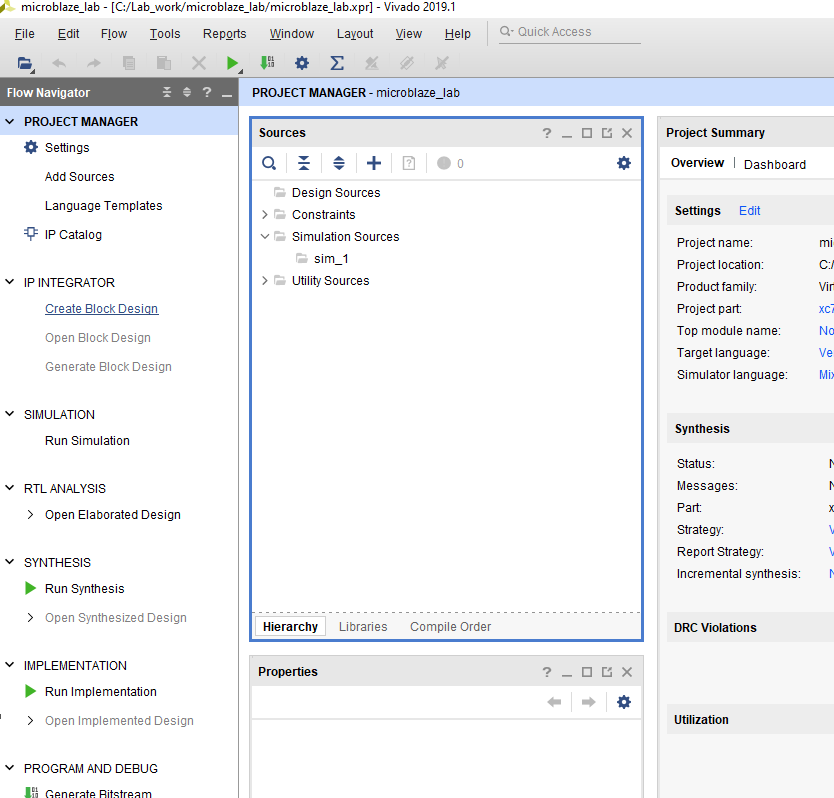
\includegraphics[scale=0.3]{image/m_12.png}   
			\label{m_12}
		\end{minipage}
	}
	\subfigure[Назначаем имя файлу] 
	{
		\begin{minipage}{8cm}
			\centering      
			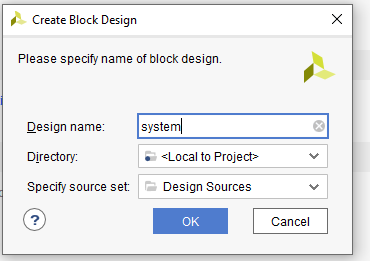
\includegraphics[scale=0.5]{image/m_13.png}   
			\label{m_13}
		\end{minipage}
	}
	\caption{Окно мастера подключения нового файла: кнопка и имя} %  %Имя большого изображения
\end{figure}

После нажатия на кнопку OK Vivado перейдёт в режим \verb|IP Integrator|.

Теперь мы можем начать собирать процессорную систему. Процесс этот во 
многом автоматизирован, и мы этим воспользуемся. Первое, что нам необходимо 
добавить в софт-процессорную систему – это сам софт-процессор MicroBlaze. Есть 
несколько вариантов его исполнения и добавления, но для проектирования таких 
простых систем, как наша, обычно используется мастер настройки. Для добавления 
IP-блоков на схему проекта (вкладка Diagram) можно воспользоваться кнопкой
Add IP или нажать Ctrl+I. После нажатия на кнопку откроется каталог блоков, которые можно 
добавить на поле Diagram.

В появившемся окне со списком доступных IP блоков (рис. ~\ref{m_16}) в поле поиска 
Search пишем MicroBlaze и выбираем из найденных позиций MicroBlaze.

Дважды кликаем по MicroBlaze, после чего IP блок появляется на поле. 
Обратите внимание, что также появилось окно настройки адресов (об этом 
позже), и «свесилась» зелёная строка помощи, которая появляется, если Vivado
может как-то автоматизировать процесс (в нашем случае появилась надпись-ссылка
Run Block Automation) и сам модуль MicroBlaze возник на поле Diagram.

\begin{figure}[!ht]
	\centering
	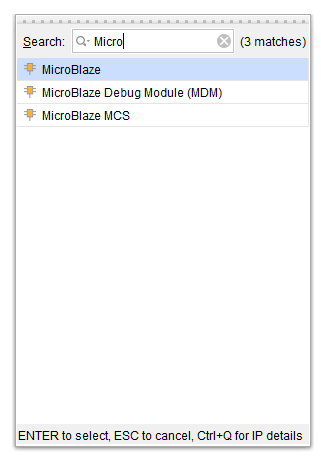
\includegraphics[width=0.3\textwidth]{image/m_16.png}
	\caption{Поиск Microblaze}
	\label{m_16}
\end{figure}

Воспользуемся автоматизацией, нажав на ссылку \verb|Run Block Automation|, после чего появится окно с мастера экспресс настроек процессорной 
системы (рис. ~\ref{m_16}). После вызова мастера доступны именно экспресс-настройки, то 
есть те, которые используются наиболее часто. Расширенные настройки доступны
по двойному щелчку на IP-блоке MicroBlaze, но это выходит за рамки текущей 
статьи.

Из предлагаемых настроек доступны:

\begin{enumerate}
    \item Количество памяти для программы и данных
    \item Управление механизмом коррекции ошибок
    \item Конфигурация кэша
    \item Конфигурация отладчика (тот самый MDM из списка)
    \item Задействование/отключение порта сопряжения с периферией (AXI-порта)
    \item Включение/выключение контроллера прерываний
    \item Выбор сигнала тактирования
\end{enumerate}

Оставим все настройки в значениях по умолчанию и нажмём кнопку OK, т. к. 
для нас этих параметров достаточно. После окончания работы мастера на поле 
появится множество новых блоков, которые мы разберём ниже. 

Как видите, картина изменилась, и на рабочем поле появились:
\begin{enumerate}
	\item Кнопка оптимизации рабочего поля
	\item Предложение по автоматическому подключению одних блоков к другим
(нажмите на неё и посмотрите, что предлагается подключить; после просмотра 
нажмите Отмена – Cancel)
      \item Блок управления тактовой частотой и синхронизацией
	\item Блок сброса процессорной системы
	\item Модуль отладки (отладчик)
	\item Ядро софт-процессора MicroBlaze
	\item Локальная память данных и программ
\end{enumerate}

\begin{figure}[!ht]
	\centering
	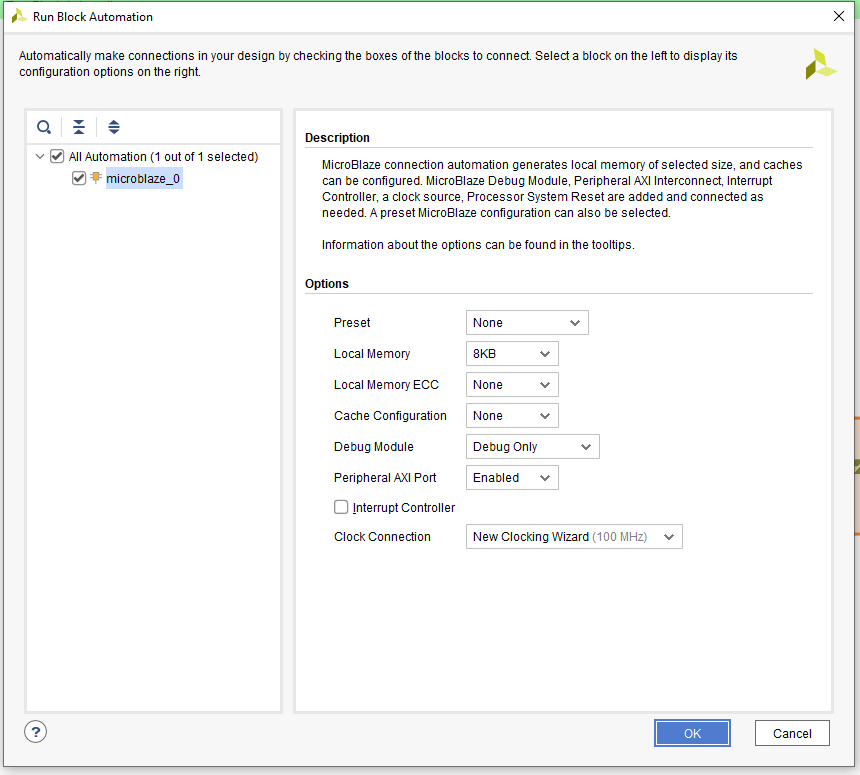
\includegraphics[width=0.4\textwidth]{image/m_18.png}
	\caption{Настройка меню Run Block Automation}
	\label{m_18}
\end{figure}

Теперь добавим необходимую периферию. В начале статьи мы определились, 
что будем мигать светодиодом, и выдавать сообщения по UART. Значит, нужно 
добавить IP-блоки, которые будут обеспечивать этот функционал. Для мигания 
будем использовать IP-блок ввода/вывода общего назначения GPIO, а для вывода сообщений – UART Lite.
Добавление IP блоков аналогично добавлению MicroBlaze. Поэтому нажимаем 
кнопку Add IP, и в поле поиска пишем gpio, выбираем модуль AXI GPIO и нажимаем 
Enter.

После добавления блока AXI GPIO необходимо его настроить, задать 
разрядность портов, определить направление и количество каналов. Настройка 
производится двойным щелчком по блоку либо выбором Customize Block из 
контекстного меню, открывающегося по щелчку правой кнопкой мыши. Модуль
\verb|axi_gpio_0| будет управлять светодиодом, периодически включая и выключая его. 
Значит \verb|axi_gpio_0| должен быть сконфигурирован следующим образом (рис. ~\ref{m_22})

\begin{enumerate}
	\item Задаём направление портов блока AXI GPIO – выбираем, что все выводы 
являются выходами, т. к. мы управляем светодиодом, а не он нами.
	\item Ставим разрядность порта 1 – всего будет подключён 1 светодиод.
	\item Второй канал нам не нужен, отключаем его.
	\item Нажимаем кнопку OK.
\end{enumerate}

Нажав плюсик около интерфейса GPIO модуля \verb|axi_gpio_0| увидим, что порт 
\verb|gpio_io_o| имеет разрядность 1 (вектор [0:0]).

Теперь давайте попробуем подключить наш настроенный блок AXI GPIO к 
MicroBlaze. Предлагаю довериться автоматике и посмотреть, что нам создаст 
Vivado. Нажимаем на строку Run connection Automation и ждём 
появления окна помощника доступных подключений (рис. ~\ref{m_24})

В окне помощника подключений:
\begin{enumerate}
	\item Выберите подключение  \verb|axi_gpio_0| и поставьте галочку \verb|S_AXI| (далее мы 
рассмотрим и поясним это подключение).
	\item Установите подключение тактового сигнала как Auto.
	\item Нажмите OK.
\end{enumerate}

После завершения подключения нажмите кнопку оптимизации рабочего 
пространства в панели инструментов.

\begin{figure}[!ht]
	\centering
	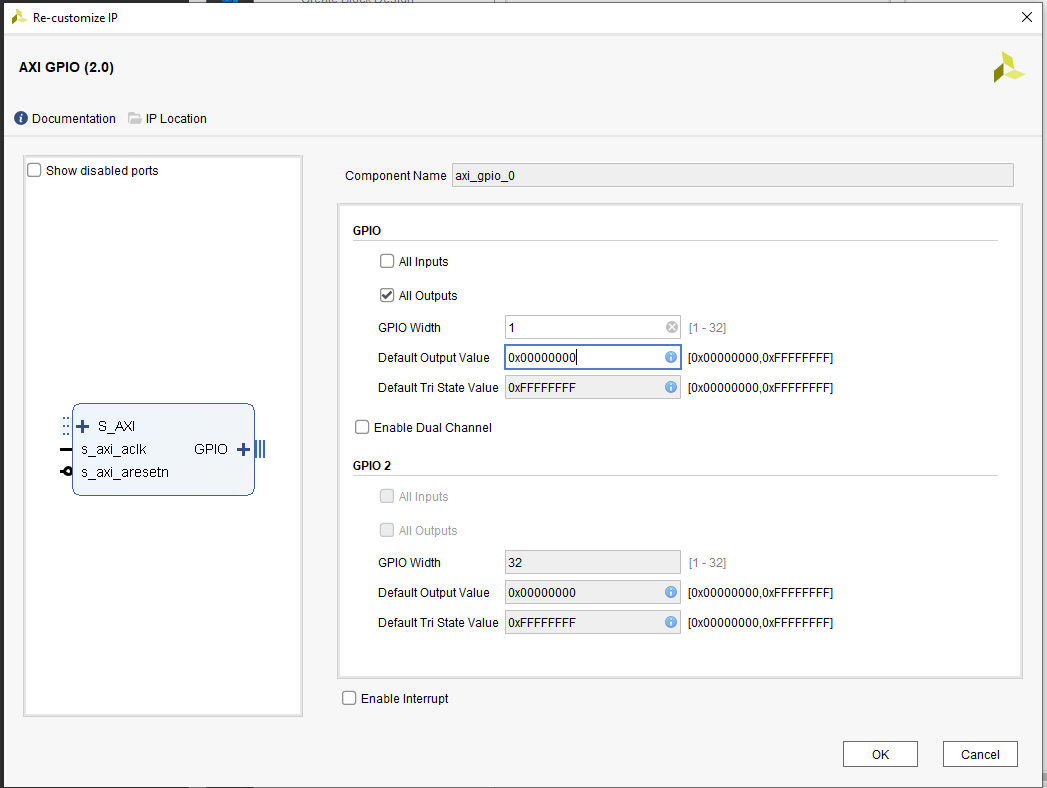
\includegraphics[width=0.4\textwidth]{image/m_22.png}
	\caption{Настройка ядра GPIO}
	\label{m_22}
\end{figure}

Как вы можете заметить, появился дополнительный модуль 
AXI Interconnect. Кратко опишем его назначение. Дело в том, что 
взаимодействие между процессором и периферией происходит по шине AXI. 
На шине есть мастер (обычно это процессор) и слэйв (Slave), в 
нашей литературе это ведущий и ведомый соответственно. Мастер отправляет 
команды слейву. Однако AXI не позволяет подключить к мастеру более одного 
слейва напрямую. Именно напрямую нельзя, но можно через коммутатор, который и 
называется AXI Interconnect – назначение этого модуля обеспечить подключение 
между несколькими мастерами и несколькими слейвами. Пока в нашей системе 
один мастер –  \verb|microblaze_0| и один слейв –  \verb|axi_gpio_0|. 

Теперь давайте попробуем добавить модуль UART Lite в нашу систему.
Надеюсь, что последовательность запомнили. Нажимаем кнопку Add IP, вводим 
в строке поиска Uartlite, дважды кликаем и ждём. 

\begin{figure}[!ht]
	\centering
	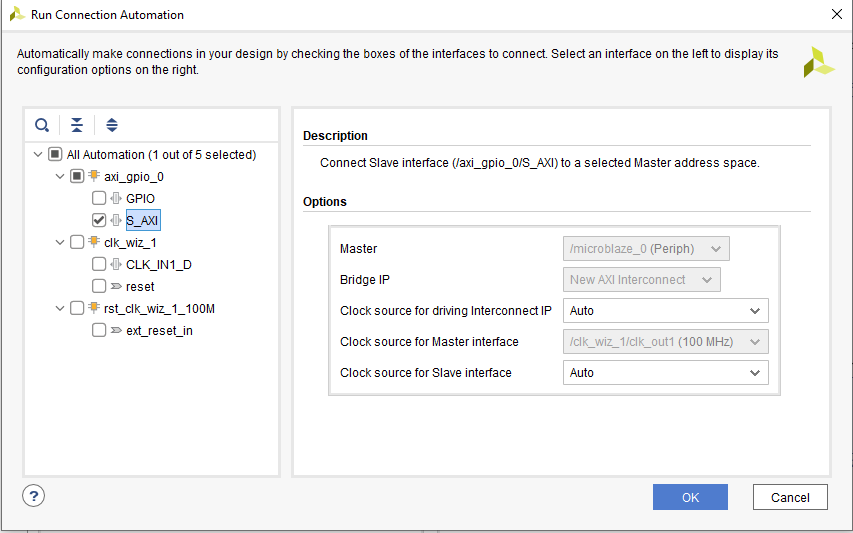
\includegraphics[width=0.4\textwidth]{image/m_24.png}
	\caption{Автоматическое подключение ядра GPIO}
	\label{m_24}
\end{figure}

При желании просмотрите доступные настройки для модуля и если есть 
необходимость, измените. Настройки обычные: скорость (9600), количество стоп
бит (1), чётность (нет), количество бит (8).
Для подключения Uartlite к нашей системе, давайте вновь воспользуемся 
автоматизацией, которую предлагает Vivado, нажав строку Run Connection
Automation. Для модуля  \verb|axi_uart_0| выберите  \verb|S_AXI| и нажмите OK (рис. ~\ref{m_28})

После завершения подключения нажмите кнопку оптимизации рабочего 
пространства и обратите внимание на изменения в AXI
Interconnect. Что произошло и почему? В AXI Interconnect добавился дополнительный 
мастер-порт для подключения второго слэйва (Uartlite – это ведомое устройство). 
MicroBlaze имеет один мастер-порт, который называется  \verb|M_AXI_DP|. Мастер один, 
а слейва два, но подключать напрямую можно только один слейв. Для подключения
нескольких слейвов мы используем AXI Interconnect. Поэтому в AXI Interconnect
добавился ещё один порт. В общем случае, AXI Interconnect может 
обеспечивать взаимное подключение нескольких мастеров и нескольких слейвов.

Теперь давайте настроим модуль управления тактовой 
частотой и синхронизацией  \verb|clk_wiz_1|. 

В окне настроек  \verb|clk_wiz_1|:
\begin{enumerate}
	\item Выберите вкладку Clocking Options.
	\item Тип модуля – MMCM.
	\item Включены возможности синтеза частоты и фазовой подстройки.
	\item Основная тактовая частота – 200MГц.
	\item Тип сигнала с системного тактового генератора на плате –
дифференциальная пара.
	\item На ней – установите выходное значение частоты (тактовая частота 
процессора) – также 100 МГц.
	\item Снимите галочку с сигнала reset.
	\item Установите галочку locked.
	\item Нажмите OK.
\end{enumerate}

Установленные настройки могут повлиять на внешний вид \verb|clk_wiz_1| (для Arty
Board он примет вид, как на рис. 29).

\begin{figure}[!ht]
	\centering
	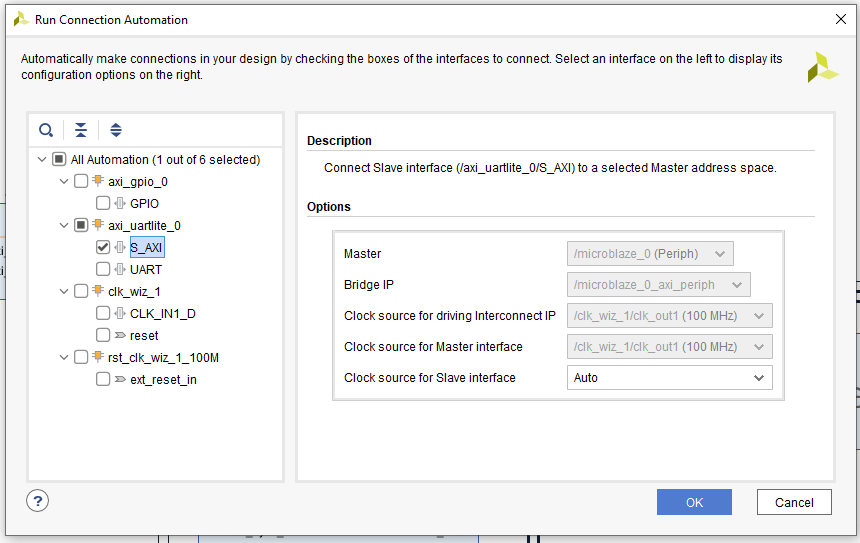
\includegraphics[width=0.7\textwidth]{image/m_28.png}
	\caption{Автоматическое подключение ядра UART}
	\label{m_28}
\end{figure}

Если оставить незадействованные выводы модуля сброса неподключенными, 
то может возникнуть ситуация, при которой процессор будет всегда в состоянии 
сброса. Потому выполним явное их подключение к логического «0» – неактивному 
для них логическому уровню. Для этого(см. рис. ~\ref{m_41}, ~\ref{m_44}):

\begin{enumerate}
	\item Добавьте блок constant.
	\item Установите в нем значение 0 (если по умолчанию оно другое).
	\item Подключите выход блока Constant к входам \verb|aux_reset_in| и  \verb|ext_reset_in|
блока \verb|rst_clk_wiz_1_100M|.
\end{enumerate}

Подключение осуществляется следующим образом: подведите мышку к 
выходу блока Constant (указатель должен принять вид карандашика), нажмите на 
выход и, не отпуская левую кнопку мыши, подведите соединение к входу 
 \verb|aux_reset_in| – а затем повторите те же действия для \verb|ext_reset_in|. В очередной раз 
нажмите кнопку оптимизации рабочего пространства в панели инструментов. 

Теперь необходимо создать внешние входы и выходы для нашей 
процессорной системы. Если вы обратили внимание, сейчас не подключены  \verb|clk_in1| 
и выходы экземпляров модулей \verb|axi_gpio_0| и  \verb|axi_uartlite_0|. Сейчас мы должны 
обозначить, какие порты являются внешними и должны выходить из нашей 
процессорной системы наружу.
Назначим вход \verb|CLK_IN1_D| модуля Clocking Wizard внешним. Для этого кликнем 
по нему правой кнопкой мыши и выберем Create Interface Port.Аналогично поступаем и с выходом GPIO модуля \verb|axi_gpio_0| и шиной UARTмодуля  \verb|axi_uartlite_0| (см. рис. ~\ref{sys_clk},~\ref{m_35},~\ref{m_37} ). 

\begin{figure}[htbp]	
	\subfigure[Тактовый сигнал] 
	{
		\begin{minipage}{8cm}
			\centering         
			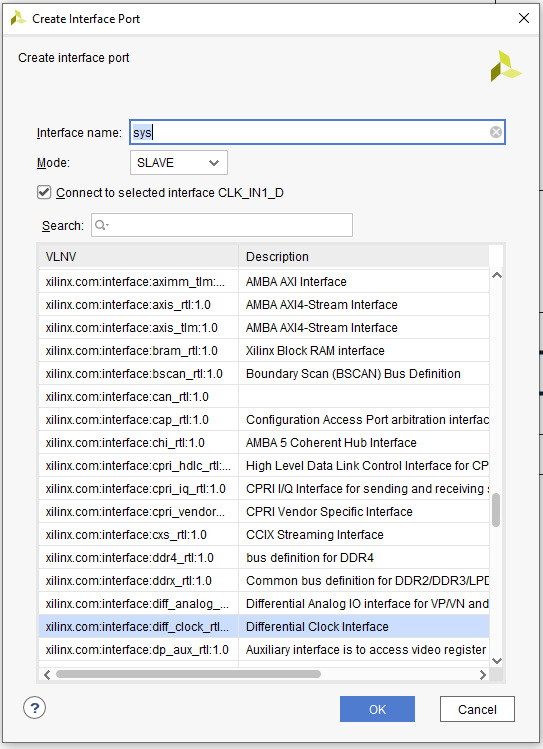
\includegraphics[scale=0.5]{image/gen.PNG}   
			\label{sys_clk}
		\end{minipage}
	}
	\subfigure[GPIO] 
	{
		\begin{minipage}{8cm}
			\centering      
			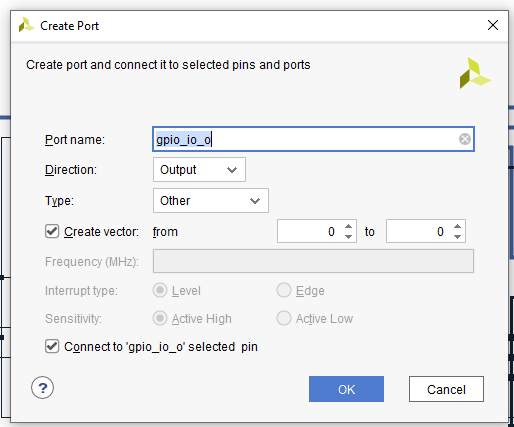
\includegraphics[scale=0.5]{image/m_35.png}   
			\label{m_35}
		\end{minipage}
	}
	\caption{Создание внешнего подключения интерфейсов: тактовый сигнал и GPIO} %  %Имя большого изображения
\end{figure}

\begin{figure}[!ht]
	\centering
	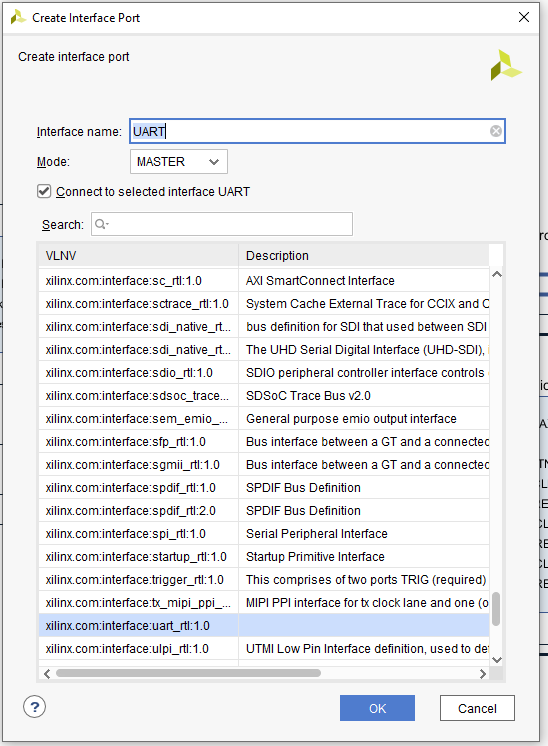
\includegraphics[width=0.3\textwidth]{image/m_37.png}
	\caption{Создание внешнего подключения интерфейса UART}
	\label{m_37}
\end{figure}

\begin{figure}[!ht]
	\centering
	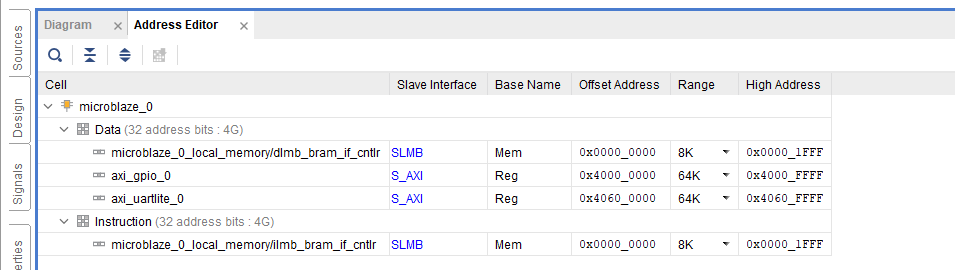
\includegraphics[width=0.8\textwidth]{image/m_39.png}
	\caption{Address Editor}
	\label{Address_Editor}
\end{figure}

Рассмотрим назначение вкладки Address Editor (рис. ~\ref{Address_Editor}).

Наши модули соединены по шине AXI, полное название AXI Memory Map, это 
значит, что все модули, подключённые к шине должны иметь уникальный адрес, 
чтобы процессор смог к ним обратиться и «не перепутать» один модуль с другим. 
Назначение уникальных адресов (распределение адресного пространства) как раз и 
происходит во вкладке \verb|Address Editor|, где в ручном, полуавтоматическом или
автоматическом режиме можно установить диапазон адресов для конкретных 
модулей.

\begin{figure}[!ht]
	\centering
	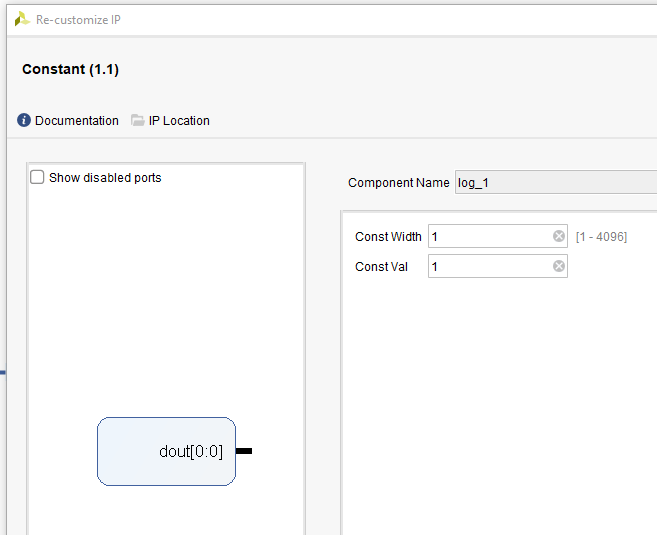
\includegraphics[width=0.4\textwidth]{image/log_1_1.png}
	\caption{Настройка Constant}
	\label{m_41}
\end{figure}

К сожалению, для нашей будущей программы не достаточно памяти, которую 
мы задали, когда пользовались мастером экспресс-настроек MicroBlaze. 
Нам необходимо увеличить количество памяти для данных и инструкций с 8К до 
16К. Сделать это можно простым выбором из выпадающего списка доступного 
количества памяти, нажав на стрелочку в соответствующем поле. Изменить 
необходимо размер памяти и инструкций. В обоих полях должно быть значение 16К.

\begin{figure}[!ht]
	\centering
	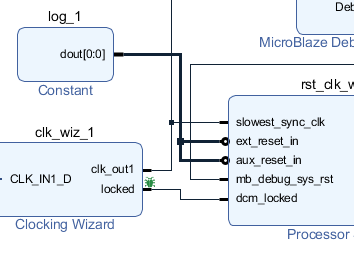
\includegraphics[width=0.4\textwidth]{image/log_1.png}
	\caption{Подключение Constant к Processor System Reset}
	\label{m_44}
\end{figure}

\begin{figure}[!ht]
	\centering
	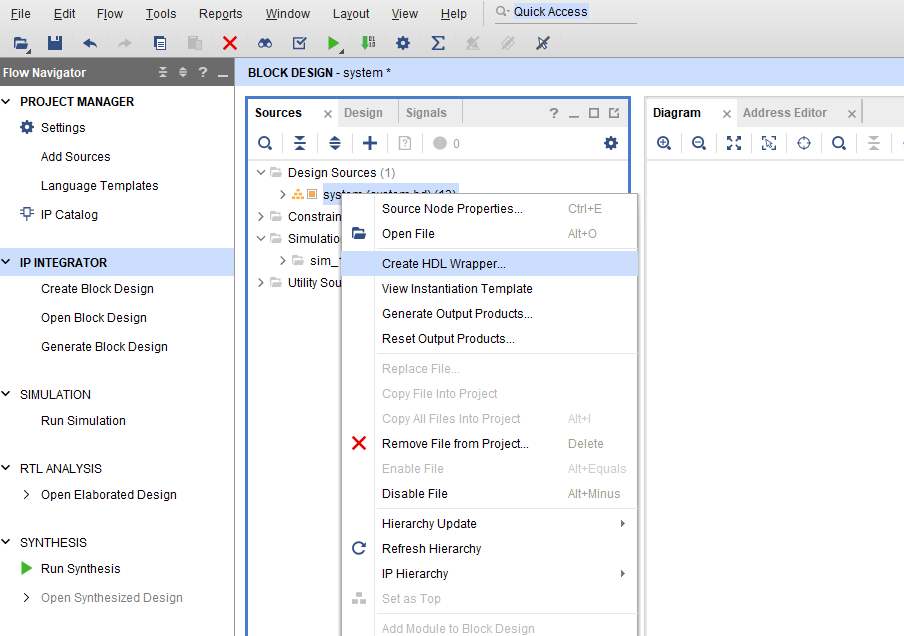
\includegraphics[width=0.4\textwidth]{image/m_46.png}
	\caption{Create HDL Wrapper: первый шаг}
	\label{m_46}
\end{figure}

Мы проделали много действий, закончили собирать систему и назначили все 
адреса. Но все ли корректно и правильно? В панели инструментов на вкладке 
Diagram есть одна из самых важных кнопок, называется она Validate Design. Нажатие этой кнопки запускает инструмент проверки 
ошибок сборки HW части процессорной системы. Нажмите эту кнопку и дождитесь результата. Если же появились ошибки – внимательно прочитайте их и постарайтесь самостоятельно исправить, вернувшись по тексту к соответствующим пунктам либо проделав всю последовательность с начала ещё раз, более внимательно и аккуратно.

\begin{figure}[!ht]
	\centering
	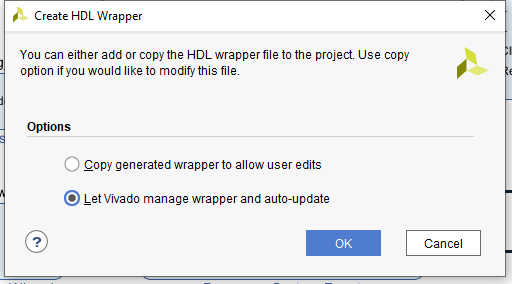
\includegraphics[width=0.4\textwidth]{image/m_47.png}
	\caption{Create HDL Wrapper: второй шаг}
	\label{m_47}
\end{figure}

Нажмите на основной панели Vivado кнопку сохранения, а затем – кнопку 
Project Manager, чтобы выйти из IP Integrator и вернуться в основной режим работы 
Vivado.

Далее следуют стандартные этапы проектирования: синтез, имплементация, 
генерация файла прошивки (битстрима). Но для блочного проекта обязательно 
нужно сделать обёртку (wrapper); это показано на рис. ~\ref{m_46},~\ref{m_47}. Нажмите правой кнопкой на созданном блочном проекте и выберите Create HDL Wrapper. В появившемся 
окне нажмите OK.

\begin{Verbatim}[tabsize=4]
# SYSCLK 200MHz
set_property PACKAGE_PIN E19 [get_ports sys_clk_p]
set_property IOSTANDARD LVDS [get_ports sys_clk_p]
set_property PACKAGE_PIN E18 [get_ports sys_clk_n]
set_property IOSTANDARD LVDS [get_ports sys_clk_n]

# LED_0
set_property PACKAGE_PIN AM39 [get_ports gpio_io_o]
set_property IOSTANDARD LVCMOS18 [get_ports gpio_io_o]

# UART
set_property PACKAGE_PIN AU33 [get_ports UART_rxd]
set_property IOSTANDARD LVCMOS18 [get_ports UART_rxd]
set_property PACKAGE_PIN AU36 [get_ports UART_txd]
set_property IOSTANDARD LVCMOS18 [get_ports UART_txd]

\end{Verbatim}

Обёртка – это простой VHDL- или Verilog-файл (с расширениями «vhd» или 
«v» соответственно), в который включена наша процессорная система, как часть 
иерархии. Таким образом, нашей собранной процессорной системой мы сможем 
оперировать, как простым модулем, добавляя её в качестве подмодуля в модули 
верхнего уровня. После создания обёртки наш модуль можно наконец-то запустить 
на синтез, нажав на кнопу Run Synthesis.

Окно, появляющееся после синтеза, предлагает выполнить:
\begin{enumerate}
	\item Запустить имплементацию.
	\item Открыть синтезируемый проект (Выберите этот пункт).
	\item Просмотреть отчёты.
\end{enumerate}
Нажмите Generate Bitstream и затем, когда Vivado предложит выполнить 
синтез и имплементацию перед запуском генерации bit-файла – нажмите Yes.
Теперь нам нужно ждать окончания генерации bit-файла. Это может занять 
минут 10-15 в зависимости от Вашего компьютера. 
По окончании генерации bit файла появится окно (рис. 50), предлагающее выполнить одно из действий. Нам 
ничего дальше делать не нужно, поэтому его просто закрываем.

\section{Проект в Xilinx SDK}

SW-часть (программная) необходима, чтобы «оживить» нашу собранную 
процессорную систему. Сейчас это просто кусок «железа», который не выполняет 
никаких действий. Как уже было сказано выше, разработка программной части 
выполнятся в среде Xilinx SDK, которая есть по сути Eclipse с плагинами от Xilinx. 
Разумеется, что Xilinx уже автоматизировал часть процесса написания программы и 
подготовил некоторые исходные файлы и библиотеки, так что писать мы будем не 
«с нуля». Сейчас нам необходимо передать Xilinx SDK информацию об аппаратной 
«начинке» нашей процессорной системы: какие использованы устройства, какова их 
конфигурация и адреса и т.д. В общем – выполнить экспорт нашей аппаратной (HW) 
части. Сделать это можно, выбрав в левом верхнем углу File -> Export -> Export Hardware
(рис. ~\ref{hw_1})

\begin{figure}[htbp]	
	\subfigure[Экспорт HW-части проекта в Xilinx SDK] 
	{
		\begin{minipage}{8cm}
			\centering         
			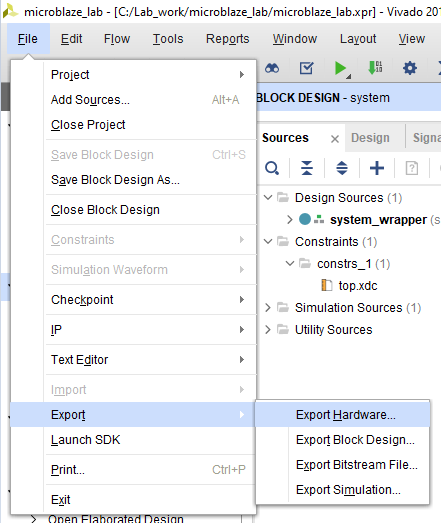
\includegraphics[scale=0.5]{image/hw_1.png}   
			\label{hw_1}
		\end{minipage}
	}
	\subfigure[Параметры экспорта HW части] 
	{
		\begin{minipage}{8cm}
			\centering      
			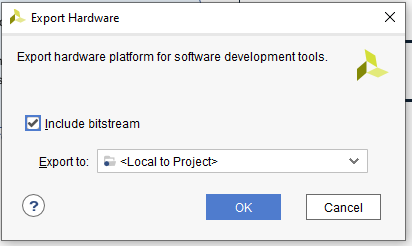
\includegraphics[scale=0.5]{image/hw_2.png}   
			\label{hw_2}
		\end{minipage}
	}
	\caption{Экспорт HW-части проекта в Xilinx SDK} %  %Имя большого изображения
\end{figure}


После этого появится окно (рис. ~\ref{hw_2}), в котором указывается, нужно ли 
экспортировать bit-файл, и какую папку выбрать в качестве рабочей. Оставим все 
настройки в состояниях по умолчанию; bit-файл экспортировать сейчас не надо, мы 
добавим его позже. Нажимаем OK.


\begin{figure}[htbp]	
	\subfigure[Назначаем проекту имя] 
	{
		\begin{minipage}{8cm}
			\centering         
			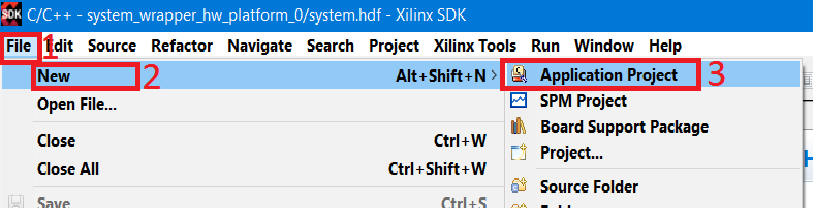
\includegraphics[scale=0.3]{image/image61.png}   
			\label{image61}
		\end{minipage}
	}
	\subfigure[Настраиваем параметры проекта] 
	{
		\begin{minipage}{8cm}
			\centering      
			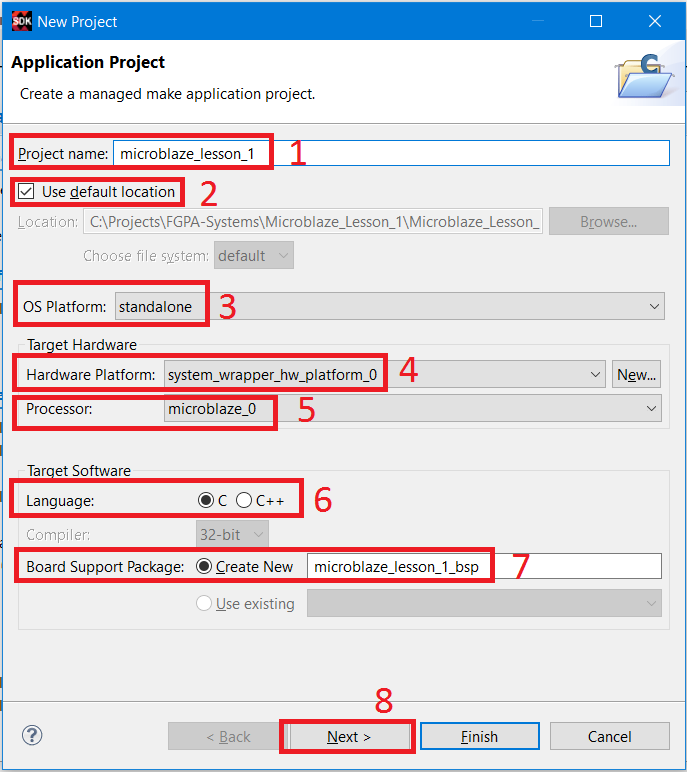
\includegraphics[scale=0.5]{image/image62.png}   
			\label{image62}
		\end{minipage}
	}
	\caption{Создание нового проекта в Xilinx SDK} %  %Имя большого изображения
\end{figure}

Теперь запускаем программу Xilinx SDK. Сделать это можно через главное 
меню Windows или из-под Vivado – просто выберите в левом верхнем углу File->Launch SDK.

Теперь Vivado просит указать параметры запуска SDK; отставим их по 
умолчанию и нажмём OK.

Приступим к созданию проекта. Выбираем File-New-Application project
Задаём основные параметры проекта (рис. ~\ref{image62}):

\begin{enumerate}
	\item Название проекта.
	\item Место расположения проекта (выставляем используемое по 
умолчанию).
	\item Тип используемой в проекте операционной системы (без ОС –
standalone).
	\item Аппаратная конфигурация (если процессоров системе несколько, то 
будет список; у нас – только один).
	\item Идентификатор процессора (актуально для многопроцессорных систем).
	\item Язык программирования (чистый C).
	\item Пакет драйверов (создаём новый на основании информации о HW части).
	\item Нажимаем Next.
\end{enumerate}

Теперь SDK предлагает выбрать один из нескольких готовых вариантов 
приложения, выбираем Hello world. После нажатия на кнопку Finish в 
проект добавляется несколько файлов и папок.

\begin{figure}[!ht]
	\centering
	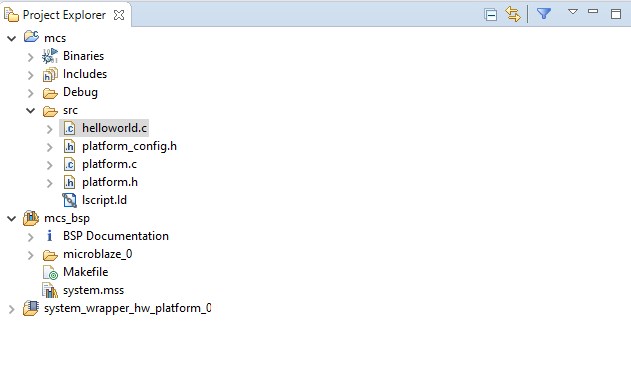
\includegraphics[width=0.5\textwidth]{image/SDK_Exp.png}
	\caption{Project Explorer в Xilinx SDK}
	\label{SDK_Exp}
\end{figure}

Откройте файл helloworld.c(см. рис. ~\ref{SDK_Exp}) и заполните его следующим кодом:

\begin{Verbatim}[tabsize=4]
#include <stdio.h>
#include "platform.h"
#include "xil_printf.h"

#include "xgpio.h"

XGpio gpio;

int main()
{
    init_platform();

    xil_printf("Hello World\n\r");

    u32 i = 0;
    u32 led = 0;
    XGpio_Initialize(&gpio, XPAR_GPIO_0_DEVICE_ID);

    while(1)
    {
    	i++;
    	if(i == 1000000)
    	{
    		led = !led;
    		XGpio_DiscreteWrite(&gpio, 1, led);
       		i = 0;
    	}
    }

    cleanup_platform();
    return 0;
}
\end{Verbatim}

После этого нажмите кнопку Build на верхней панели. 

\begin{figure}[htbp]	
	\subfigure[Настройка->COM-порт...] 
	{
		\begin{minipage}{8cm}
			\centering         
			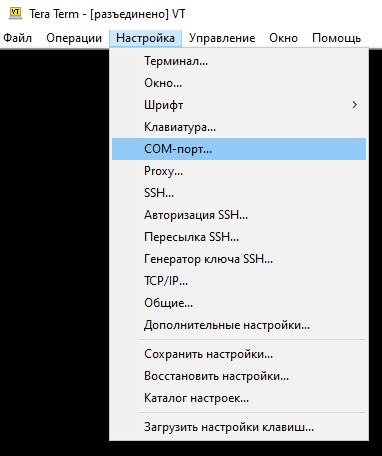
\includegraphics[scale=0.5]{image/Terra_0.png}   
			\label{terra_wind}
		\end{minipage}
	}
	\subfigure[Terra Term: Serial Port and Setup Connection] 
	{
		\begin{minipage}{8cm}
			\centering      
			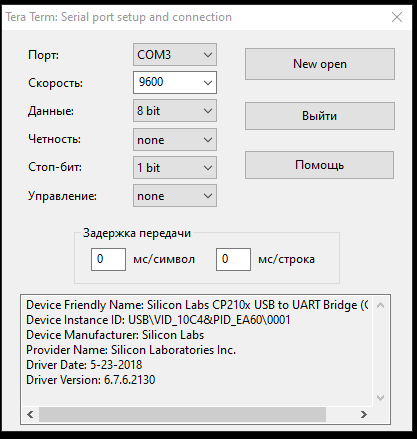
\includegraphics[scale=0.5]{image/terra.png}   
			\label{terra_com}
		\end{minipage}
	}
	\caption{Настройка программы Terra Term} %  %Имя большого изображения
\end{figure}

Перед тем как прошивать ПЛИС настроим Terra Term для просмотра сообщений переданных по UART от софт-процессора(см. рис. ~\ref{terra_wind}, ~\ref{terra_com}).
После успешной сборки проекта и настройки Terra Term можно прошивать ПЛИС. Для этого нажмите Program FPGA(см. рис. ~\ref{program_FPGA}).

\begin{figure}[!ht]
	\centering
	\includegraphics[width=0.5\textwidth]{image/program_FPGA.png}
	\caption{Program FPGA в Xilinx SDK}
	\label{program_FPGA}
\end{figure}

В результате прошивки ПЛИС нулевой светодиод на плате VC707 должен начать мигать, а в Terra Term должно появиться сообщение «Hello, world!»(см. рис. ~\ref{terra_result}).

\begin{figure}[!ht]
	\centering
	\includegraphics[width=0.5\textwidth]{image/terra_result.png}
	\caption{Результаты вывода сообщения в консоль}
	\label{terra_result}
\end{figure}

\newpage

Задачи:

\begin{enumerate}
	\item Сделайте бегущие огни из восьми светодиодов, которые установлены на отладочной плате VC707.
	\item Настройте ядро GPIO таким образом, что бы можно было считывать состояния кнопок, установленных на плате, и отображать их состояние в Terra Term.
\end{enumerate}

Вопросы:

\begin{enumerate}
	\item Как работает ядро Processor System Reset? В какой последовательности и с какими задержками оно формирует сброс?
	\item Какой формат пакета имеет интерфейс UART?
	\item Какие регистры есть у ядра AXI UARTLite? Нарисуйте структурную схему данного ядра.
\end{enumerate}